\documentclass[modern]{aastex631}

\usepackage{amsmath}

\begin{document}

\title{A Practical Line Cleaner for Narrow Lines in Gravitational Wave Data}

\author[0000-0003-1540-8562]{Will M. Farr}
\email{will.farr@stonybrook.edu}
\email{wfarr@flatironinstitute.org}
\affiliation{Department of Physics and Astronomy, Stony Brook University, Stony Brook, NY 11794, USA}
\affiliation{Center for Computational Astrophysics, Flatiron Institute, New York, NY 10010, USA}

\begin{abstract}
    Blah
\end{abstract}

\section{Theory}
\label{sec:theory}

Consider a simple harmonic oscillator driven by a stochastically-fluctuating
signal, $n(t)$,
\begin{equation}
    \ddot{x}(t) + 2\gamma\dot{x}(t) + \left( 2 \pi f_0 \right)^2 x(t) = n(t),
\end{equation}
with damping rate $\gamma$ and natural angular frequency $\omega_0$.  In the
Fourier domain, the solution satisfies the algebraic equation 
\begin{equation}
    -\left( 2 \pi f \right)^2 X(f) + 4 \pi i\gamma f X(f) + \left( 2 \pi f_0 \right)^2 X(f) = N(f),
\end{equation}
or
\begin{equation}
    X(f) = \frac{N(f)}{\left( 2 \pi f_0 \right)^2 - \left( 2 \pi f \right)^2 + 4 \pi i\gamma f},
\end{equation}
if we ignore the free, homogeneous solutions to the differential equation (which
anyway must damp out over timescales $\tau \gg \gamma^{-1}$).  If $n$ is
wide-sense stationary and zero-mean, then 
\begin{eqnarray}
    \left\langle N \right\rangle & = & 0, \\
    \left\langle N^*(f)N(f') \right\rangle & = &
    S_n(f) \delta(f - f'),
\end{eqnarray}
for some (positive) function $S_n$, called the power spectral density of the
noise $n$.  This implies 
\begin{eqnarray}
    \left\langle X \right\rangle & = & 0, \\
    \left\langle X^*(f)X(f') \right\rangle & = & \frac{S_n(f)}{\left(\left( 2 \pi f_0 \right)^2 - \left( 2 \pi f \right)^2\right)^2 + 16 \pi^2 \gamma^2 f^2}\delta(f - f') \equiv S_x(f) \delta\left( f - f' \right).
\end{eqnarray}
If, furthermore, $n$ is Gaussian distributed, then $x$ will be as well,
following an independent Gaussian distribution at each frequency $\omega$ with
mean and variance indicated above.  Many narrow-band features (lines) in
gravitational wave data can be adequately described by this model.  

Assuming $\gamma / f_0 \ll 1$, over short timescales $\tau$ that are longer than
the natural period associated to the solution, but short compared to the damping
time, i.e.\ $f_0^{-1} \ll \tau \ll \gamma^{-1}$, the solution is sinusoidal with
frequency $f_0$.  Over longer timescales the solution oscillates at the natural
frequency, but with random \emph{phases}. For some lines in present-day
gravitational wave detectors, the damping time is much longer than the analysis
segments of typical signals; in such cases, it is possible to use data from
before and after (and during) the analysis segment to \emph{infer} the phase of
the line through the analysis segment and \emph{regress} it out of the data,
improving the signal-to-noise ratio of the signal.  This is the basic idea
behind the line cleaner described in this note.

Given a stretch of data in the (discrete) Fourier domain from a total
observation time $T$, 
\begin{equation}
    D_k \simeq D\left( f = \frac{k}{T} \right) = \frac{T}{N} \sum_{n=0}^{N-1} d_n e^{-2\pi i k n / N},
\end{equation} 
and restricting our attention to a narrow range of frequencies $f_l < f < f_h$
around a line that we want to regress, it is reasonable to assume that the data
are a sum of the line and some background, continuum noise; we can assume that
the background noise power spectrum, $S_0$, is constant because the bandwidth is
narrow. Then the likelihood for the data $D$ given the line contribution $X$ is 
\begin{equation}
    p\left( D_k \mid X_k, S_0 \right) = N\left( D_k \mid X_k, \sqrt{T S_0} \right).
\end{equation}
(In words: the data are normally distributed with mean $X$ and standard
deviation $\sqrt{T S_0}$.)  It is also reasonable to assume that the
line-driving noise spectrum $S_n$ is constant over the narrow bandwith; we have
seen above that the line itself is normally distributed with mean zero and
variance $S_x(f) T$, so 
\begin{equation}
    p\left( X_k \mid S_n, f_0, \gamma \right) = N\left( X_k \mid 0, \sqrt{S_x\left(f_k \mid S_n, f_0, \gamma \right) T} \right).
\end{equation}
The product of these two normal distributions is, itself a normal distribution;
and it can be factorized in various ways \citep{Hogg2020}.  One factorization
writes it as a product of the marginal likelihood for the data given line
parameters and continuum noise,
\begin{equation}
    p\left( D_k \mid S_n, f_0, \gamma, S_0 \right) = N\left( D_k \mid 0, \sqrt{S_x\left(f_k \mid S_n, f_0, \gamma \right) T + S_0 T} \right);
\end{equation}
and the conditional posterior for the line $X_k$ given the data and parameters 
\begin{multline}
    p\left( X_k \mid D_k, S_n, f_0, \gamma, S_0 \right) \\ = N\left( X_k \mid \frac{S_x\left(f_k \mid S_n, f_0, \gamma \right) D_k}{S_x\left(f_k \mid S_n, f_0, \gamma \right) + S_0}, \sqrt{\frac{S_x\left(f_k \mid S_n, f_0, \gamma \right) S_0 T}{S_x\left(f_k \mid S_n, f_0, \gamma \right) + S_0}} \right).
\end{multline}

Applying a prior on the line and continuum parameters, and using standard
stochastic sampling techniques (MCMC, HMC, etc) allows to explore the posterior
over $S_n$, $f_0$, $\gamma$, and $S_0$ given data; for each sample, we can then
draw the line $X_k$ from the conditional posterior above.  

Subtracting a fair draw of the line from the data generates a residual sample, 
\begin{equation}
    R_k \equiv D_k - X_k,
\end{equation}
which can then be passed to downstream data analysis pipelines.  We choose to
pass onward a fair sample of the residuals instead of, say, the maximum
likelihood residuals so that the noise properties of the residuals are
un-biasedly described by the spectral density $S_0$; see Appendix
\ref{sec:oversubtract}.

\section{Implementation}

TODO.

\begin{figure}
    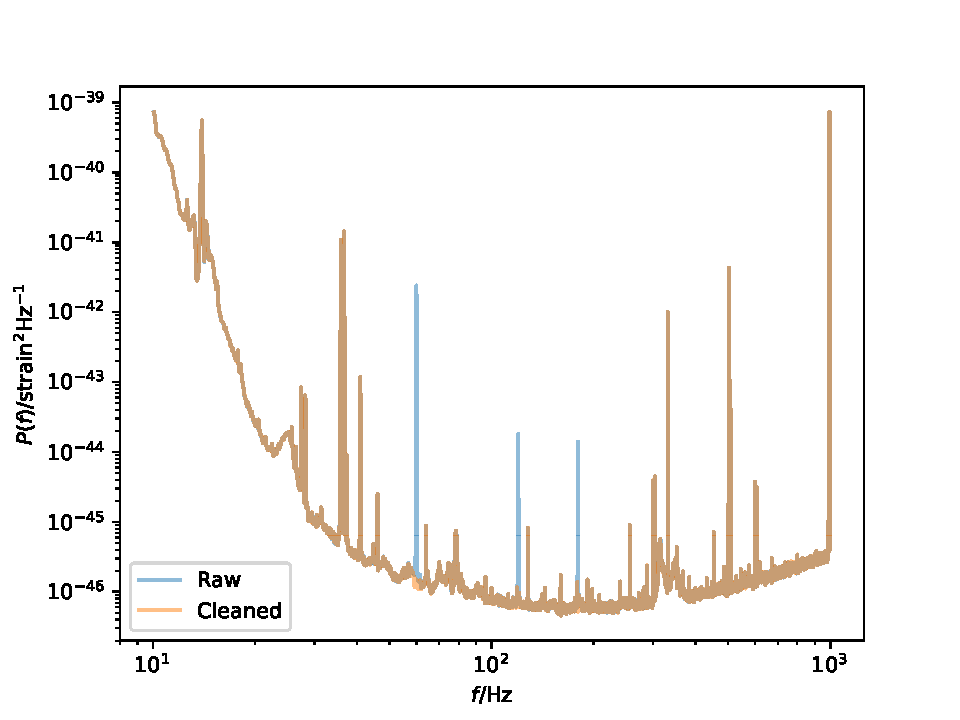
\includegraphics[width=\columnwidth]{raw-and-cleaned-psd.pdf}
    \caption{\label{fig:cleaned-psd} An example of a cleaning of data from the Hanford LIGO observatory around the GW150914 event \cite{Abbott2016,Abbott2019,GWOSC,GWOSC2,GW150914-GWOSC}.  The Lorentzian lines at $60 \, \mathrm{Hz}$, $120 \, \mathrm{Hz}$, and $180 \, \mathrm{Hz}$ are clearly visible in the raw data, but are removed by the line cleaner; the cleaning used $4 \, \mathrm{Hz}$ bandwidth around each line.  Figure \ref{fig:line-zoom} shows the raw and cleaned data in the vicinity of each line.}
\end{figure}

\begin{figure}
    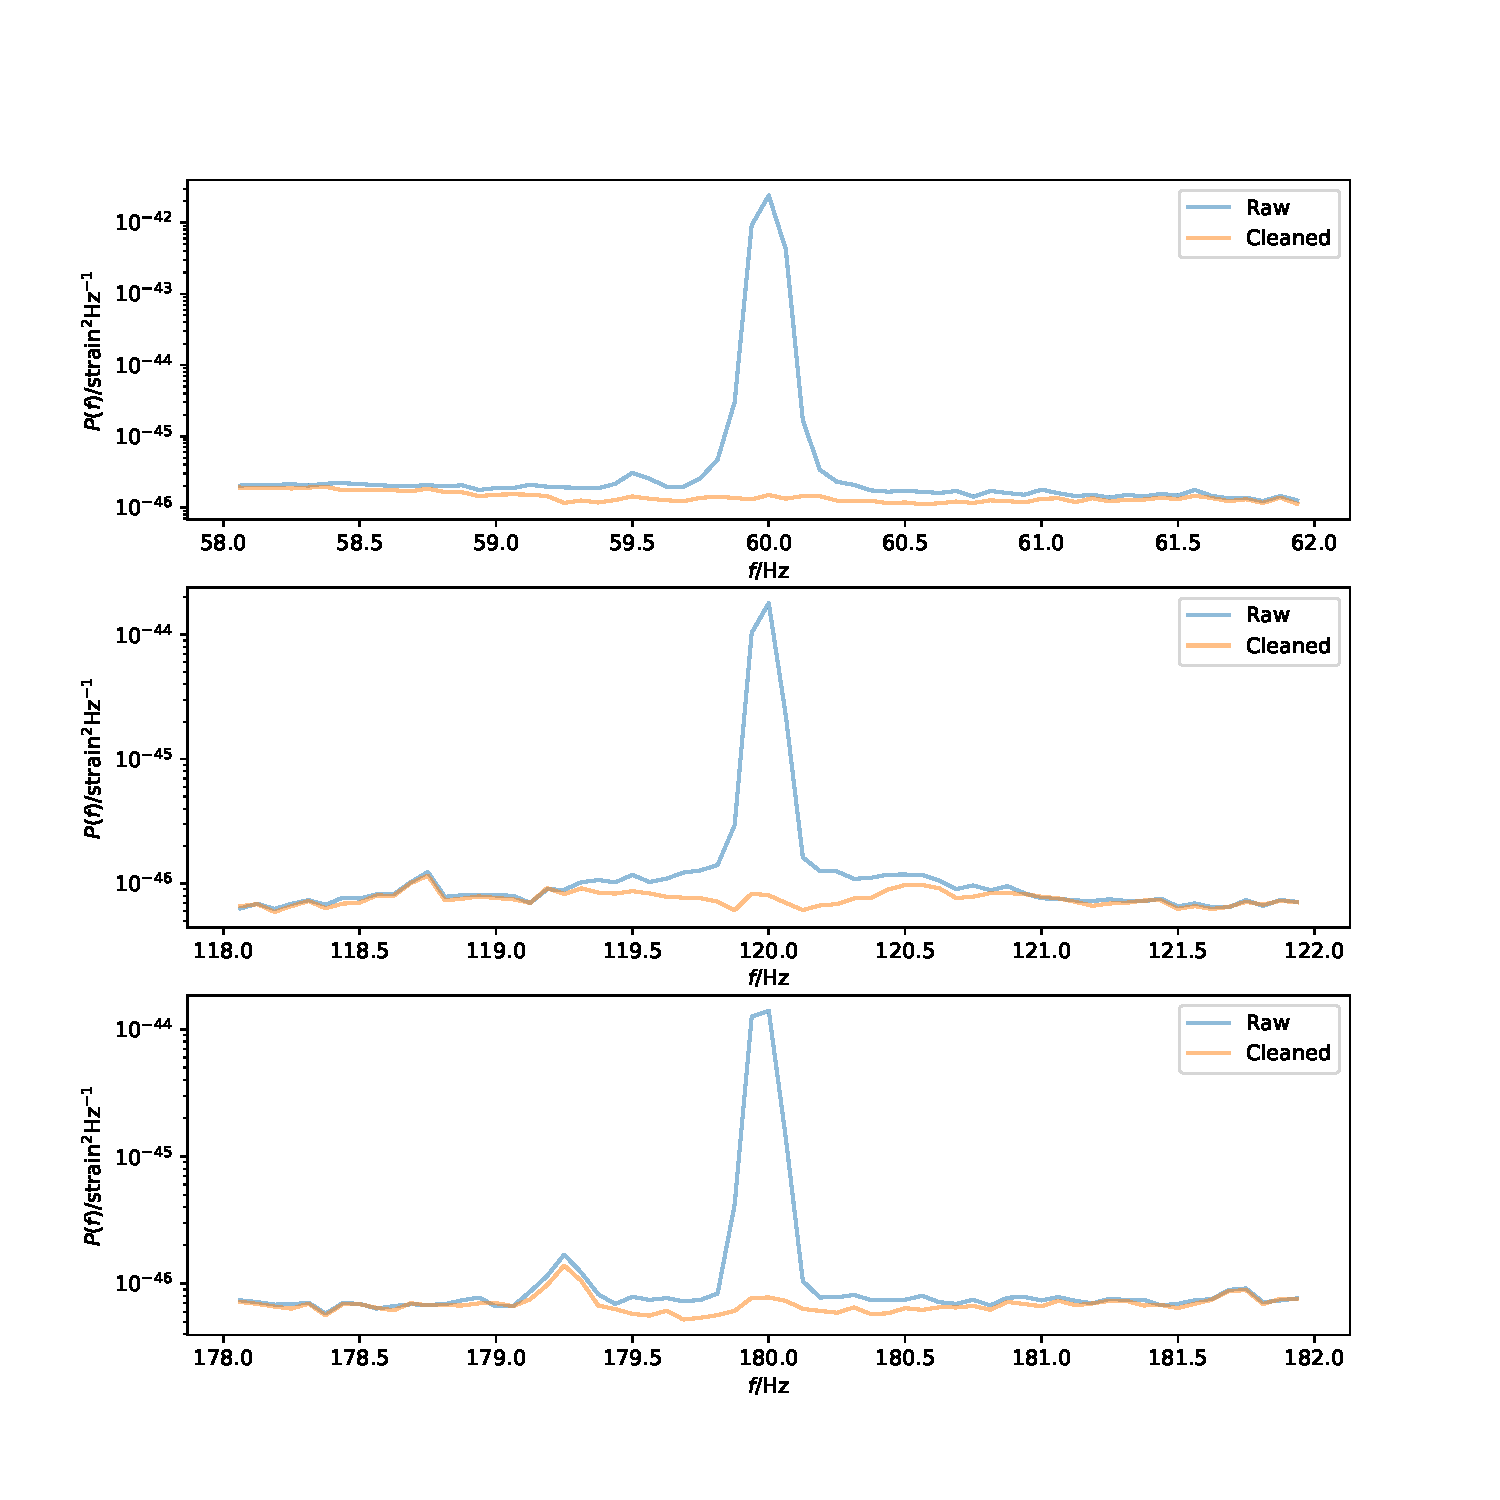
\includegraphics[width=\columnwidth]{line-zoom-in.pdf}
    \caption{\label{fig:line-zoom} A zoom-in of the raw and cleaned data shown in Figure \ref{fig:cleaned-psd}.}
\end{figure}

\appendix

\section{Avoiding Over-Subtraction}
\label{sec:oversubtract}

As discussed in Section \ref{sec:theory}, the line cleaner algorithm subtracts a
fair draw from the posterior over the line parameters and line values, instead
of using the maximum-likelihood values for either of these quantities.  This
procedure avoids oversubtraction of the line, which is particularly important if
downstream analyses are producing, for example, a noise estimate from the
residuals.

Before showing these results.

\bibliographystyle{aasjournal}
\bibliography{linecleaner}

\end{document}